% This is samplepaper.tex, a sample chapter demonstrating the
% LLNCS macro package for Springer Computer Science proceedings;
% Version 2.21 of 2022/01/12
%
\documentclass[runningheads]{llncs}
%
\usepackage[T1]{fontenc}
% T1 fonts will be used to generate the final print and online PDFs,
% so please use T1 fonts in your manuscript whenever possible.
% Other font encondings may result in incorrect characters.
%
\usepackage{graphicx}
% Used for displaying a sample figure. If possible, figure files should
% be included in EPS format.
%
% If you use the hyperref package, please uncomment the following two lines
% to display URLs in blue roman font according to Springer's eBook style:
%\usepackage{color}
%\renewcommand\UrlFont{\color{blue}\rmfamily}
%\urlstyle{rm}
%

% Olivier
\usepackage{changepage}

\begin{document}
%
\title{New Schema Mechanisms for Developmental Artificial Intelligence}
%
\titlerunning{Schema Mechanisms}
% If the paper title is too long for the running head, you can set
% an abbreviated paper title here
%
\author{Olivier L. Georgeon\inst{1}\orcidID{0000-0003-4883-8702} \and
Filipo Perotto\inst{2} \and
Arash Shekhlar\inst{3} \and
Paul Robertson\inst{4}\orcidID{0000-0002-4477-0379}
}
%
\authorrunning{Georgeon, Perotto, Schekhlar \& Robertson}
% First names are abbreviated in the running head.
% If there are more than two authors, 'et al.' is used.
%
\institute{UR CONFLUENCE: Sciences et Humanites (EA 1598), UCLy, France \email{ogeorgeon@univ-catholyon.fr}\\
\and ONERA, France \email{filipo.perotto@onera.fr}
\and Center for Analysis and Design of Intelligent Agents, Reykjavik University, Iceland \email{arashs@ru.is}
\and DOLL Labs, Lexington, MA, USA\\ \email{paulr@dollabs.com}
 }
%
\maketitle              % typeset the header of the contribution
%
\begin{abstract}
Schema mechanisms are software systems that attempt to account for the learning theories that are designated under vocable such as genetic epistemology, constructivist epistemology, and developmental learning.  
The works of Jean Piaget constitute the central body of reference of these theories ranging from child psychology to philosophy of mind.
Gary Drescher coined the term schema mechanism in 1991 and laid the ground to identifying the core challenges: open-ended learning, intrinsic motivation, incremental hierarchical abstraction, sensorimotor grounding, reflexivity, individuation. 
%he modeled Piagetian sensorimot schemas as datastructures that encompass sensory data and actions, 
This paper reviews a selection of the latest schema mechanisms and highlights their contributions to these key challenges, with the goal of unifying their different contributions toward a comprehensive theory of developmental artificial intelligence.

\keywords{Schema mechanism  \and Genetic epistemology \and Constructivist learning.}
\end{abstract}
%
%
%
\section{Introduction}


Drawing from the earlier work of James Baldwin, Jean Piaget developed and popularized the theory of \textit{genetic epistemology} \cite{piaget_principles_1997} throughout his life to account for the genesis of intelligence and knowledge. 
In the end of his life, he connected genetic epistemology with constructivist epistemology and the work of Ernst von Glasersfeld \cite{glasersfeld_radical_1997}. 
Genetic epistemology rests on the key concept of ``scheme'' which Piaget defines as follows: 
\\

\begin{adjustwidth}{1cm}{1cm}
``A scheme is a structure or organization of actions as they transfer or generalize in similar or analogous circumstances.'' 
(\cite{piaget_naissance_1998}, p. 23).
\\ 
\end{adjustwidth}

In this paper, we translate \textit{scheme} with the English term \textit{schema} and its plural \textit{schemas}. 
A schema is the basic unit of knowledge that encapsulates the action and its circumstances, that is, a \textit{pattern of interaction}. 
Genetic epistemology insists on the primacy of interaction as a condition for the emergence of perception and knowledge:
\\

\begin{adjustwidth}{1cm}{1cm}
``Knowledge does not originally arise either from a subject conscious of itself or from objects already constituted (from the subject's point of view) that would impose themselves on the subject. 
Knowledge results from interactions occurring halfway between the subject and the objects, and thus involving both, but due to a complete un-differentiation and not from exchanges between distinct forms.

If, at the beginning, there is neither a subject, in the epistemic sense of the term, nor objects, conceived as such, nor, above all, invariant instruments of exchange, then the initial problem of knowledge will be to construct such mediators. 
Starting from the contact zone between one's own body and the objects, these mediators will progressively engage more deeply in both complementary directions toward the exterior and the interior. 
It is from this dual progressive construction that the joint elaboration of both the subject and the objects depends.

The initial instrument of exchange is not perception, as rationalists too easily conceded to empiricism, but rather action itself, with its much greater plasticity. 
Certainly, perceptions play an essential role, but they partly depend on action as a whole, and some perceptual mechanisms that one might have thought to be innate or very primitive only emerge at a certain level of object construction.'' (translated from \cite{piaget_lepistemologie_2011}, p14-15)
\\

\end{adjustwidth}


Guerin and McKenzie \cite{guerin_survey_2013} proposed Fig. \ref{fig:general} to picture the progressive organization of schemas as the infant develops.

\begin{figure}
	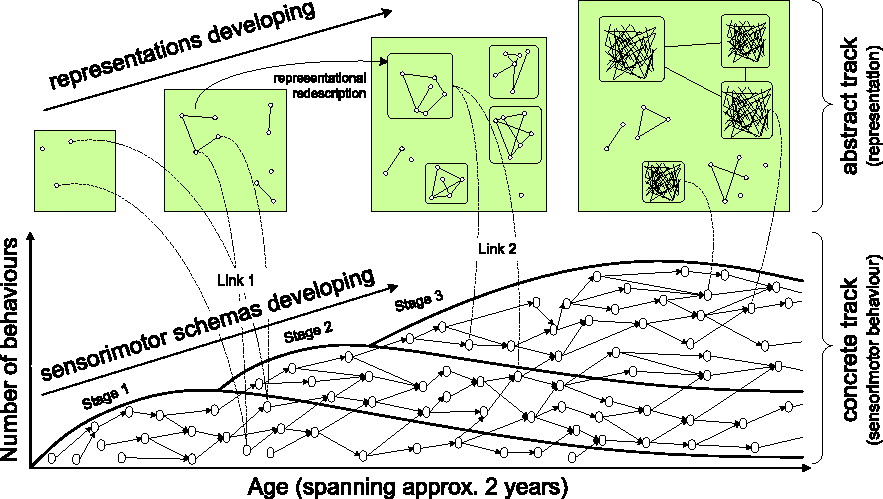
\includegraphics[width=\textwidth]{Figure_1_guerin.pdf}
	\caption{Conceptual diagram of infant development from \cite{guerin_survey_2013} Fig. 1.
	The lower (concrete) track shows a directed acyclic graph of sensorimotor schemas. 
	A node represents a newly created schema. 
	An edge has the meaning ``is a necessary precursor''. 
    Stage 1: behaviors without objects. 
    Stage 2: behaviors with single objects. 
    Stage 3: object-object behaviors. The schemas now involve relationship among objects, and locations and transforms within space.
    The higher (abstract) track represents representations of objects by schemas and physical properties influencing their interactions.} 
	\label{fig:general}
\end{figure}

Ziemke \cite{ziemke_construction_2001} examined how these views apply to robotics.
Oudeyer \cite{oudeyer_intrinsic_2007} stressed the importance of intrinsic motivation. 


\section{Schema mechanisms}

Drescher \cite{drescher_made-up_1991} pioneered the first schema mechanism by modeling schemas as a tuple (context, action, result) depicted in Fig. \ref{fig:drescher}. 
A schema's context is satisfied when all the positively included items are \textit{On} and all the negatively included items are \textit{Off}. 
The activation is a schema consists of initiating its action. An activated schema is said to \textit{succeed} if its predicted results are all in fact obtained, and to \textit{fail} otherwise. The ratio of success and failure is called \textit{reliability} and is memorized for each schema.  
Schemas can be chained to achieve goals. 

\begin{figure}
	\centering
	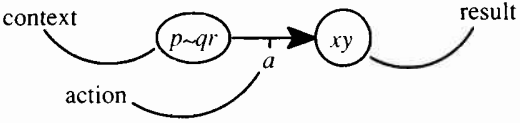
\includegraphics[width=0.6\textwidth]{Figure_2_schema_drescher.png}
	\caption{Schema from \cite{drescher_made-up_1991} Fig. 3.2.
	The schema noted $p \!\sim\! qr/a/xy$ asserts that if action $a$ is taken in the context where item $p$ is On, $q$ is Off, and $r$ is On then the items $x$ and $y$ will be turned On.} 
	\label{fig:drescher}
\end{figure}

\cite{drescher_made-up_1991}
\cite{chaput_constructivist_2004}
\cite{guerin_piagetian_2008}
\cite{wang_new_2012}
\cite{miller_building_2018}

\subsection{Perotto's}

Similar to Drescher's, Perotto's schemas \cite{perotto_computational_nodate} are tuples that associate a context, an action, and an expected result. 
Perotto, however, introduces a new distinction between two kinds of context variables: hidden variables and observable variables as shown in  Fig. \ref{fig:perotto}.

\begin{figure}
	\centering
	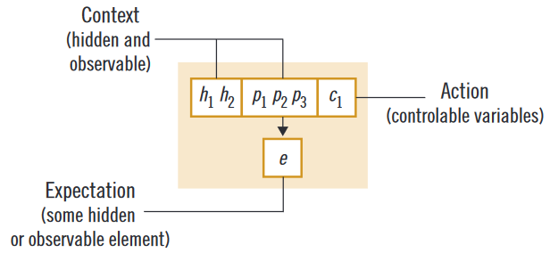
\includegraphics[width=0.6\textwidth]{Figure_perotto.png}
	\caption{Perotto's schema from \cite{perotto_computational_nodate} Fig. 2.
		A schema is composed of three vectors: context containing hidden variables and observable properties $(h_1, h_2, p_1, p_2, p_3)$, action $(c_1)$, and expected result $(e)$. } 
	\label{fig:perotto}
\end{figure}

Perotto also introduced a hierarchy of schemas called the \textit{anticipatory tree} represented in Fig. \ref{fig:perotto_tree}. 
Schema are organized in the \textit{anticipatory tree} whose top-level schema describes the agent's highest-level goal and leaf schemas are deciders of actions in the environment.

\begin{figure}
	\centering
	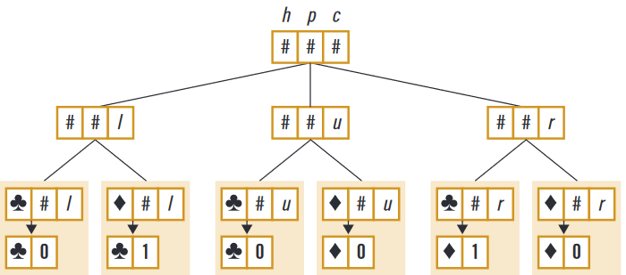
\includegraphics[width=0.7\textwidth]{Figure_perotto_tree.png}
	\caption{Example of Perotto's anticipatory tree from \cite{perotto_computational_nodate} Fig. 10: ``Final schematic tree for solving the flip problem.''.
 } 
	\label{fig:perotto_tree}
\end{figure}



\subsection{AERA}

AERA is a causality-based general machine intelligence aspiring system with the following components \cite{sheikhlar2024causal,nivel2013replicode}: 

\noindent \textbf{Facts}: Facts are statements that represent an entity’s property and property’s value at a time step.

\noindent \textbf{Composite state ($CST$)}: A composite state represents a set of simultaneous facts the AERA system considers to be significant for predicting an event’s consequences.

\noindent \textbf{Command model ($CoM$)}: A command model represents a causal influence of an event on the state of the AERA agent’s environment, i.e., a change in the value of an entity’s property at a later time step.

\noindent \textbf{Requirement model ($M_{req}$)}: A requirement model allows a $CoM$ to be instantiated after its relevant CST is instantiated.

Figure \ref{fig:AERA} shows how the above components lead to making a prediction. When some observation facts match all the components of a $CST$, the $CST$ will be instantiated through a $M_{req}$ which itself leads to the instantiation of a $CoM$. As the $CoM$ predicts a future state after an event’s occurrence, the AERA agent verifies if the observation facts in the following time step match the predicted state.

\begin{figure}
	\centering
	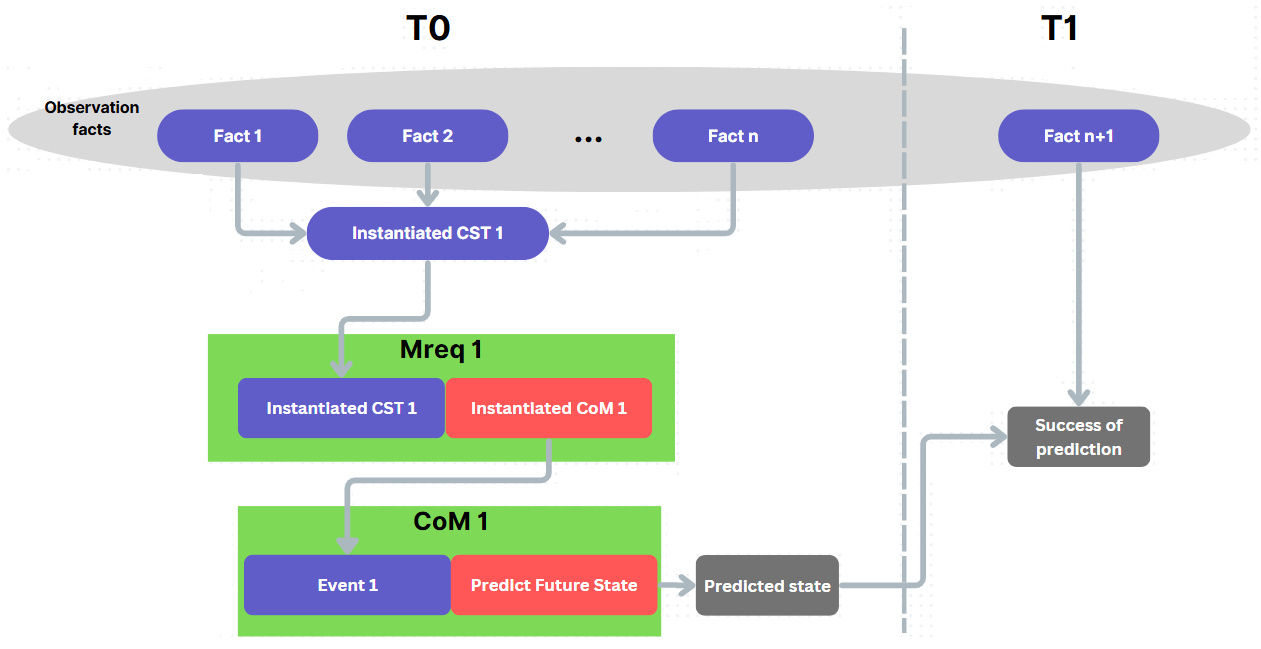
\includegraphics[width=0.99\textwidth]{AERAblockdiagram.png}
	\caption{ The connection between a $CST$, a $CoM$, and a $M_{req}$ in AERA. } 
	\label{fig:AERA}
\end{figure}

The differences between AERA’s knowledge representation and Drecher’s schemas have to do with AERA following the rules of non-axiomatic logic and its support for higher-order logic. In other words,
\begin{itemize}
    \item The models in AERA are falsifiable, have degrees of confidence, and can be related to specific groups with certain attributes specifying their context.
    \item The choice of models and reasoning in AERA is based on the extent of available resources (models and time).
    \item The knowledge representation in AERA is compositional, meaning that AERA can create hierarchies of models and composite states.
\end{itemize}

Yet, both AERA models and schemas represent knowledge in a similar manner, they contextualize the statements representing an action/event's consequences. 


\subsection{The LIDA cognitive architecture}

The LIDA cognitive architecture \cite{kugele_learning_2021}  implements a schema mechanisms on top of a perceptual memory module called the Perceptual Associative Memory (PAM). Percepts are not directly received from the environment but constructed in the PAM through an active sensorimotor process. 

\begin{figure}
	\centering
	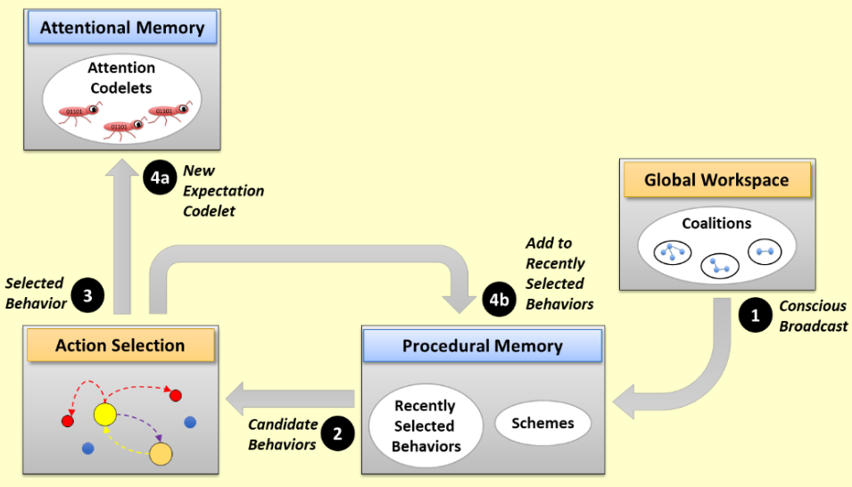
\includegraphics[width=0.7\textwidth]{Figure_LIDA1.png}
	\caption{Initiation of LIDA's procedural learning process (\cite{kugele_learning_2021} Fig. 10)} 
	\label{fig:lida1}
\end{figure}

\begin{figure}
	\centering
	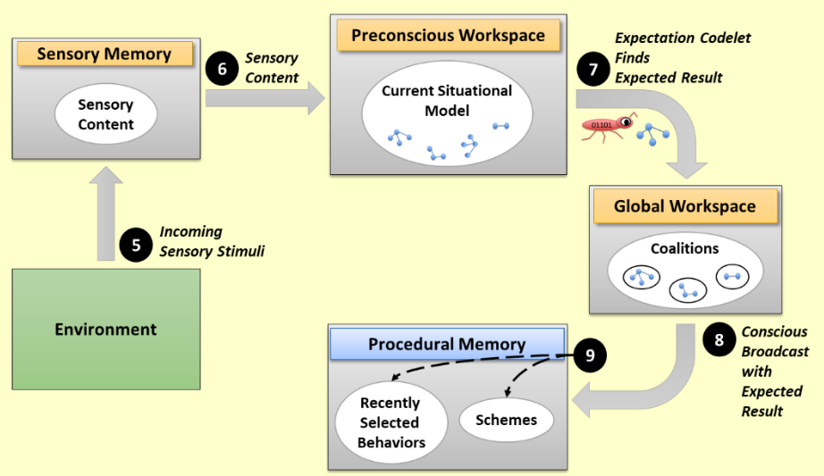
\includegraphics[width=0.7\textwidth]{Figure_LIDA2.png}
	\caption{Continuing process of selectionist and instructionalist procedural learning that was initiated by Action Selection (\cite{kugele_learning_2021} Fig. 11)} 
	\label{fig:lida2}
\end{figure}


\subsection{Georgeon's}

Similar to Perotto, Georgeon modeled schemas as tuples (pre-condition, decision, post-condition), and organized them  hierarchically. 

In contrast with Drescher's and Perotto's mechanisms, however, pre-conditions and post-conditions are not properties of the world (hidden or observed) but are other schemas learned previously. 
The mechanism learns new schemas from the bottom up, with higher-level schemas made of a sequence of two previously-learned lower-level schemas, 
as illustrated in Fig. \ref{fig:agent8}. 
The mechanism is not initialized with a top-level goal. 
Instead, it is initialized with a predefined set of low-level primitive schemas that define the agent's basic possibilities of interaction. 
In a robot, primitive schemas are hard-coded control loops involving actuators and sensory feedback. 


\begin{figure}
	\centering
	\includegraphics[width=1.0\textwidth]{Figure_3_agent8.pdf}
	\caption{Schema learning and selection.
		Schemas are nested tuples: (pre-schema, decision, post-schema).
		Over time, new decisions and new schemas are learned from the bottom up. 
		Recently enacted schemas (in gray) activate the previously-learned higher-level schema whose pre-schema they match.
		Activated schemas propose their post-schemas with a proclivity value calculated from the activation weight and the expected valence.
		The schema with the highest proclivity is selected to try to enact.} 
	\label{fig:agent8}
\end{figure}


The schema learning mechanism and selection works as follows.
At the end of time step $t$, the agent records or reinforces the schemas: 
\begin{itemize}
	\item[$\bullet$] $(i_{t-2}, d_{t-1}, i_{t-1})$
	\item[$\bullet$] $((i_{t-3}, d_{t-2}, i_{t-2}), d_{t-1}, i_{t-1})$
	\item[$\bullet$] $(i_{t-3}, d^2, (i_{t-2}, d_{t-1}, i_{t-1}))$
	\item[$\bullet$] $((i_{t-4}, d_{t-3}, i_{t-3}), d^2, (i_{t-2}, d_{t-1}, i_{t-1}))$
\end{itemize}

If it does not yet exist, the new decision $d^2$ is constructed different from the decision $d_{t-2}$ that was actually made at time $t-2$. 
For example, if the agent made decision $d_{t-2} = a0$ and enacted interaction $i_{t-2}=i00$, and then made decision $d_{t-1} = a0$, and enacted interaction $i_{t-1}=i01$, the agent learns the new decision $d^2=i00a0$ consisting of trying to enact the interaction $i_t=i00$ and then do action $a_{t+1}=a0$. 
When decision $d^2$ has been selected and successfully enacted, the mechanism learns higher-level schemas on top of it. 
The rate of schema construction being constant, the number of schemas grows linearly with time. 
Older and unused schemas can be forgotten.

In essence, the agent learns habits of interaction that are organized hierarchically, with shorter sequential habits learned first, and longer sequences of habits made of sequences of shorter habits later learned on top of them. 
Such habit learning relates to Woolford's \textit{sensorimotor sequence reiterator} \cite{woolford_precarious_2020}.

\section{Benchmarks}
\label{sec:benchmarks}

Fig. \ref{fig:drescher2} shows Drescher's experimental settings.


\begin{figure}
	\centering
	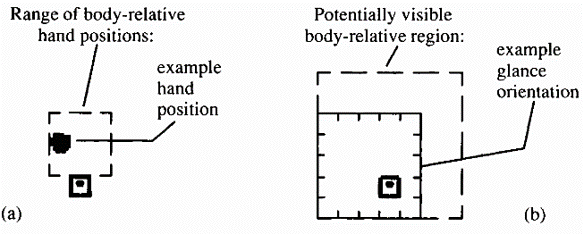
\includegraphics[width=0.6\textwidth]{Figure_drescher_expe.png}
	\caption{Drescher's benchmark from \cite{drescher_made-up_1991} Fig.6.1 ``Hand and glance ranges''.} 
	\label{fig:drescher2}
\end{figure}

Fig. \ref{fig:perotto_ben} shows Perotto's experimental settings \cite{perotto_computational_nodate}.


\begin{figure}
	\centering
	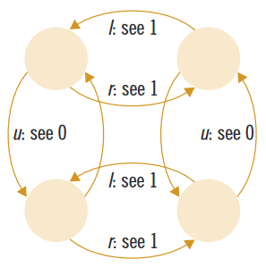
\includegraphics[width=0.3\textwidth]{Figure_perotto_benchmark.png}
	\caption{Perotto's benchmark from \cite{perotto_computational_nodate} Fig.9 ``The hyper-flip problem''.} 
	\label{fig:perotto_ben}
\end{figure}


\begin{figure}
	\centering
	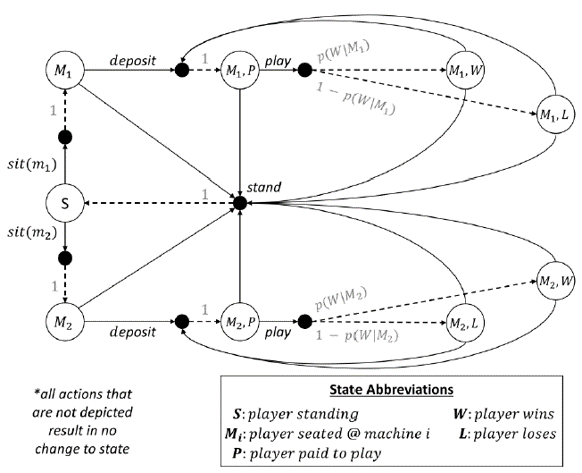
\includegraphics[width=0.7\textwidth]{Figure_LIDA_bench.png}
	\caption{The multi-armed bandit environment used to assess LIDA's schema Mechanisms (\cite{kugele_constructivist_nodate} Fig. 5)} 
	\label{fig:lida_bench}
\end{figure}



Fig. \ref{fig:georgeon} shows Georgeon' experimental settings \cite{georgeon_intrinsically-motivated_2012}.
Video Demo \cite{georgeon_video_2012}.


\begin{figure}
	\centering
	
\includegraphics[width=0.3\textwidth]{Figure_grid_plot.pdf}
	\caption{Georgeon's benchmark (Adapted from \cite{georgeon_intrinsically-motivated_2012}).
	The agent can move forward to an empty cell, bump into a wall (green cell), turn to the left or to right by 90°, or ``feel'' the cell in front, to the left, or to the right. 
	Sensory signal is a single-bit feedback from the action. 	
} 
	\label{fig:georgeon}
\end{figure}


\section{Schema mechanisms and theory of knowledge}

Bettoni  has criticized Drescher's schema mechanism in stating that ``Drescher's Constructivism is not Piaget's Constructivism, mainly because of its tacit acceptance of \textit{cognitive dogmatism}'' (\cite{bettoni_made-up_1993}, p. 6).
Bettoni describes cognitive dogmatism as taking for granted that ``patterns and structures of objects, attributes, relations, etc. [...] be as much as possible true copies of `original' objects, attributes, relations etc. in the world'' (\cite{bettoni_made-up_1993}, p. 1).
Indeed, theories of enaction as well as of radical constructivism have insisted that we should not take the sensory signals as representational items of an alleged reality. 


The game of Mastermind provides an emblematic example in which the observation is not representational. 
Player 2 attempts to infer a hidden combination of colored pegs (``hidden state'') by proposing guesses (``actions''), which Player 1 responds to with feedback pegs (``observation''). Black pegs indicate a correct color in the correct position, while white pegs indicate a correct color in the wrong position.
Since the observation depends on the action, there exist no function or stochastic distribution that map the state to the observation. 
The absence of such function or distribution is expressed in cognitive terms by that the observation is not ``representational'' of the state.

Software to play Mastermind have been proposed using diverse techniques such as entropy measure and evolutionary algorithms \cite{cotta_entropy-driven_2010}.
These techniques, however, require that the semantics of the feedback is known beforehand. 
We propose the \textit{constructivist Mastermind analogy} that likens a general learner to someone playing a giant game of mastermind where they start with no knowledge of the hidden combination and even the semantics of actions and feedback.
The player may never find the hidden combination or goal but may survive and strive for some time in a satisfactory \textit{knowledge niche}.

As reviewed in Section \ref{sec:benchmarks}, most schema mechanisms have been tested in settings in which the sensory signal is representational.
Nonetheless, the fact that they have not been tested with non-representational sensory signal does not mean that they would not work or could not be adapted to such settings. 
Georgeon's mechanism may constitute an illustration of that.  
In Georgeon's schemas, the sensory data is feedback from action rather than beeing representational. 
The pre-condition and post-condition of schemas are are just other schemas all the way down to non-representational primitive schemas. 
In essence, the agent knows its current context by possibilities of interaction rather than by representational data. 

Georgeon's schema mechanism is not targeted at reaching a predefined goal. Since sensory data does not represent the environment's state, the agent cannot have a goal represented as an environment state. Instead, the agent's behavior is driven by the expected valence of each decision. 
The calculation of expected valence may incorporate predefined preferences for some primitive schemas or different intrinsic motivation principles such as an estimation of information gained. 


\section{Conclusion}

Beyond the first stage called by Piaget the \textit{sensorimotor level}, comes a second stage he calls the \textit{first level of pre-operative thought} (\cite{piaget_lepistemologie_2011}, p. 30). 
It is at this second stage that the subject begins to differentiate itself from the objects. 
The subject becomes able to manipulate the schemas by thought. 
Piaget formulates this process as follows: 
\\

\begin{adjustwidth}{1cm}{1cm}
``On top of simple actions that ensure direct interdependence between the subject and objects, in certain cases, a new type of action is superimposed, one that is internalized and more precisely conceptualized: for example, in addition to being able to move from A to B, the subject acquires the ability to mentally represent this movement from A to B and to evoke, through thought, other movements'' (translated from \cite{piaget_lepistemologie_2011}, p. 30).\\

\end{adjustwidth}

Future studies on schema mechanisms will have to address this second stage to tackle fundamental questions of knowledge abstraction. 
We expect this will involve a cognitive architecture that has the capacity to represent spatial properties of schemas, and to simulate the enaction of schema in different spatial frames of reference. LIDA and ECA \cite{georgeon_artificial_2024} constitute initial attempts in this direction . 


\begin{credits}
\subsubsection{\ackname} .

\subsubsection{\discintname}
The authors have no competing interests to declare that are
relevant to the content of this article.
\end{credits}
%
% ---- Bibliography ----
%
% BibTeX users should specify bibliography style 'splncs04'.
% References will then be sorted and formatted in the correct style.
%
\bibliographystyle{splncs04}
\bibliography{ConstructivistAI.bib}
%
\end{document}
